% =====================================================================
% Scientific Data Data Descriptor — Drought Intelligence Explorer v2.0.0
% Standalone LaTeX: embedded numerical references, no .bib/.bbl dependency.
% Compile: latexmk -pdf manuscript.tex
% =====================================================================
\documentclass[11pt,a4paper]{article}
\usepackage[utf8]{inputenc}
\usepackage[a4paper,left=0.55in,right=0.55in,top=0.70in,bottom=0.70in]{geometry}
\usepackage{graphicx}
\usepackage{booktabs}
\usepackage{tabularx}
\usepackage{array}
\usepackage{ragged2e}
\usepackage{longtable}
\usepackage{xcolor}
\usepackage{caption}
\usepackage{enumitem}
\usepackage[protrusion=true,expansion=false]{microtype}
\usepackage[numbers,sort&compress,super]{natbib}
\usepackage[hyphens]{url}
\usepackage{hyperref}
\hypersetup{hidelinks,pdftitle={A three-era district drought data resource for India spanning 1901 to 2100},pdfauthor={Ankit Deshmukh}}
\graphicspath{{figures/}}
\setlength{\parskip}{4pt}
\setlength{\parindent}{0pt}
\setlength{\emergencystretch}{3em}
\makeatletter
\setlength{\@fptop}{0pt}
\setlength{\@fpbot}{0pt plus 1fil}
\makeatother
\setcounter{topnumber}{3}
\setcounter{bottomnumber}{2}
\setcounter{totalnumber}{4}
\renewcommand{\topfraction}{0.92}
\renewcommand{\bottomfraction}{0.60}
\renewcommand{\textfraction}{0.06}
\renewcommand{\floatpagefraction}{0.75}
\renewcommand{\arraystretch}{1.18}
\setcitestyle{numbers,sort&compress,super}
\DeclareCaptionLabelSeparator{pipe}{ $|$ }
\captionsetup{font=small,labelfont=bf,labelsep=pipe,skip=6pt}
\renewcommand{\figurename}{Fig.}

\begin{document}

{\LARGE\bfseries A three-era district drought data resource for India spanning 1901 to 2100\par}
\vspace{10pt}
{\large Ankit Deshmukh\textsuperscript{1}\par}
\vspace{4pt}
{\small\textsuperscript{1}Department of Civil Engineering, Pandit Deendayal Energy University, Gandhinagar, Gujarat, India\par}
\vspace{3pt}
{\small Correspondence: deshmukh.acad@gmail.com \quad ORCID: \url{https://orcid.org/0000-0002-1433-3872}\par}
\vspace{12pt}

\section*{Abstract}
Drought research in India requires consistent records that combine spatial detail, several drought indicators and transparent provenance. We present a monthly district-level resource for 724 districts in 36 States and Union Territories, organised into three labelled eras that are never spliced. The gridded multi-source era contains ten indicators derived from CHIRPS precipitation, ERA5-Land evapotranspiration and soil moisture, and MODIS vegetation from January 1981 to September 2026. The reconstruction era contains SPEI at 1-, 4- and 12-month scales from 1901 to 2025. The projections era contains bias-corrected CMIP6 simulations for 2015--2100 under two shared socioeconomic pathways, with ensemble spread and model agreement. Missing values are not imputed. The resource includes versioned Parquet files, wide CSV matrices, metadata, validation products and a browser-based SQL engine. Technical checks include deterministic pipeline tests, an independent India Meteorological Department benchmark, reconstruction--gridded overlap comparisons and committed climate-model release gates. Software and data are archived under persistent identifiers for reuse in drought climatology, model evaluation, teaching and secondary analysis.

\section*{Background \& Summary}
Drought is a domain-dependent climate hazard. Meteorological, agricultural, hydrological and socio-economic drought respond to deficits over different time scales, and no single index represents all of them\citep{WilhiteGlantz1985,MishraSingh2010}. The Standardized Precipitation Index (SPI) describes accumulated precipitation anomalies on a chosen time scale\citep{McKee1993}. The Standardized Precipitation Evapotranspiration Index (SPEI) applies comparable probability machinery to precipitation minus potential evapotranspiration and therefore also responds to atmospheric evaporative demand\citep{VicenteSerrano2010}. Vegetation and soil-moisture indicators describe aspects of the land-surface response\citep{Kogan1995}. International guidance consequently recommends multiple indices and time scales rather than a single drought number\citep{WMOLincoln2009}.

India presents a demanding setting for such a record. Rainfall is concentrated in a strongly seasonal monsoon and varies sharply across space, while agriculture, water resources and ecosystems respond on different delays. The India Meteorological Department (IMD) provides gridded rainfall and temperature products\citep{Pai2014,Srivastava2009} and operational drought information. The National Remote Sensing Centre publishes vegetation-based agricultural drought assessments. The Drought Atlas of India supplies a high-resolution, long-term SPEI reconstruction\citep{Chuphal2024,ChuphalData2024}. These products answer different questions. Operational services emphasise current conditions; the Atlas provides archive depth but one indicator family; and a researcher seeking several indicators at a stable district scale must otherwise assemble and document a new processing chain.

The resource described here integrates data, processing, validation and access in one citable contract. It covers 724 administrative districts in 36 States and Union Territories and contains three explicitly labelled eras (Fig. 1). Era A is the Drought Atlas reconstruction for 1901--2025, containing SPEI-1, SPEI-4 and SPEI-12. Era B is a gridded multi-source product for January 1981--September 2026, containing SPI-1/3/6/12, SPEI-1/3/6/12, a root-zone soil moisture anomaly (SMA) and the Vegetation Condition Index (VCI); its ten matrices contain 3,780,163 valid district-month values. Era C contains bias-corrected CMIP6 simulations for 2015--2100 under SSP2-4.5 and SSP5-8.5. The eras share district identifiers and a long-format schema, but retain separate source, reference-period and uncertainty labels and are never combined into an unqualified historical series.

Version 2.0.0 extends the previously published version 1.0.0 resource\citep{DeshmukhV1Data2026}. Era A, era C, the cross-validation products and the query engine are new to this descriptor; era B preserves the published indicator semantics and monthly refresh policy while extending the record through September 2026. The contribution is therefore integration and validation rather than the invention of new drought indices. Public inputs include CHIRPS precipitation\citep{Funk2015}, ERA5-Land\citep{MunozSabater2021}, MODIS vegetation indices\citep{Didan2015}, the Drought Atlas\citep{ChuphalData2024} and CMIP6 simulations\citep{Eyring2016,ONeill2016}. Established SPI/SPEI definitions, quantile delta mapping\citep{Cannon2015} and Hargreaves--Samani potential evapotranspiration\citep{HargreavesSamani1985} are used throughout.

The processing chain is designed to make each published value traceable. Source composites are area-weighted to districts; index fits are checked against their base samples; missing observations remain missing; event, trend and relationship rules are fixed in configuration and code; and derived files carry checksums and provenance. Version 2.0.0 of the software\citep{DeshmukhSoftware2026} and its companion dataset\citep{DeshmukhData2026} are archived under persistent identifiers. The browser application exposes maps, charts, district profiles, event and trend analyses, SQL queries and reproducibility-headed exports without an account or backend.

The data support secondary analyses of drought frequency, duration, severity, seasonality, indicator relationships and model performance. They are not operational drought declarations. Projections are simulations rather than forecasts, reconstructions and reanalysis are not in-situ observations, and district aggregates do not acquire the native resolution of their source grids. These distinctions are retained in the metadata, interface, figures and archive.

\begin{figure}[t]
\centering
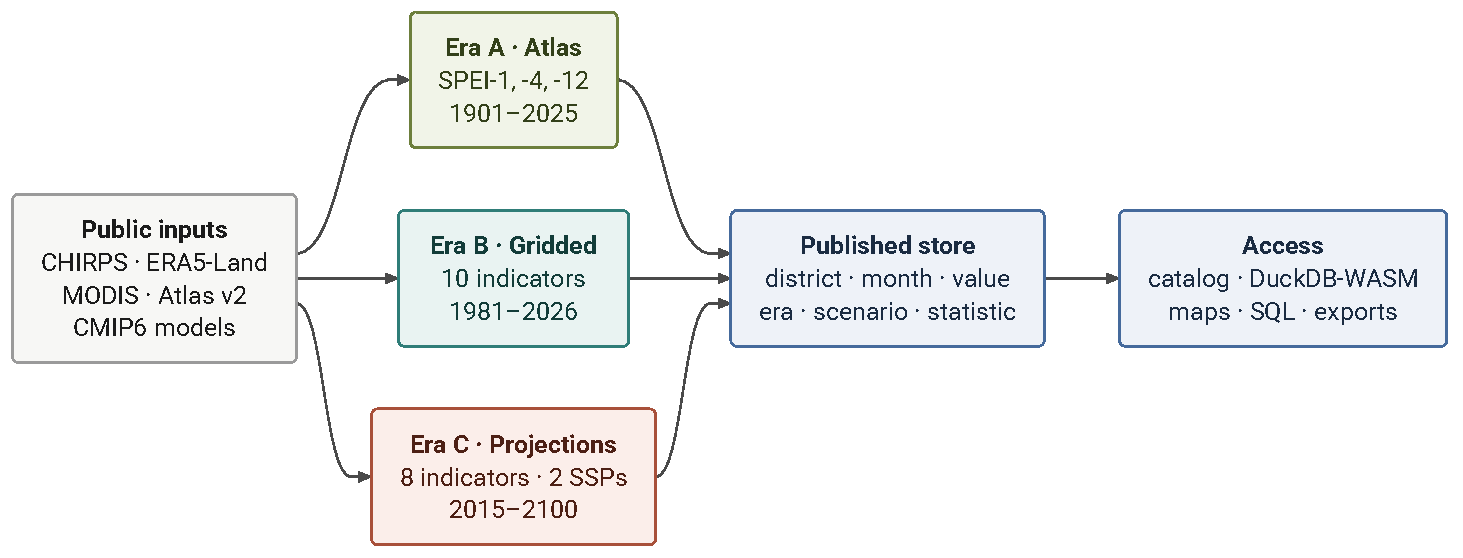
\includegraphics[width=\textwidth]{fig01_architecture.pdf}
\caption{Three-era record architecture. Era A is a reconstruction, era B is a gridded multi-source product and era C contains model simulations. Each era is processed onto the same 724-district reporting fabric and published through a common long-format schema, while era, source, scenario, statistic and reference-period labels remain explicit. Record windows are distinguished from the 1981--2020 standardisation reference and the 1981--2014 cross-era comparison window. Missing observations are represented by absent rows and are never imputed.}
\end{figure}

\section*{Methods}

\subsection*{Study area and spatial units}
The reporting units are 724 unique district polygons across 36 States and Union Territories from the community \path{india-maps-data} repository\citep{uditIndiaMaps}. The source uses a 2011-era demarcation lineage and includes some units created after the 2011 census. The published fabric is deliberately fixed over the full record. Later district reorganisations are not crosswalked because no validated spatio-temporal allocation is available, and reallocating historical values across changing vintages would introduce an additional source of error.

All regional areas and area-weighted summaries use a Lambert Azimuthal Equal-Area (LAEA) projection centred at 22.5$^\circ$N, 79.5$^\circ$E. The served district fabric totals 3,266,386~km$^2$, approximately 0.64\% below India's published area. The shortfall is primarily a property of the source geometry rather than the web simplification; its decomposition is reported in Technical Validation. Boundaries are not authoritative for legal purposes and follow the depiction of the source dataset. The source repository does not declare an explicit redistribution licence. Boundary files are therefore attributable, separable from the indicator matrices and accompanied by the source disclaimer; users requiring a formally licensed geometry can substitute another fabric with a documented crosswalk.

District values are area aggregates of gridded fields, not point measurements. Native resolution remains approximately 0.05$^\circ$ for CHIRPS and the Atlas, 0.1$^\circ$ for ERA5-Land and 1~km for MODIS. Small districts can depend on few source pixels, and neighbouring district estimates are not statistically independent. The reporting fabric and native source grids are documented in Data Records and illustrated in the interface figures.

\subsection*{Input datasets}
Table 1 lists the input products, versions, access routes and terms. Era B was produced through Google Earth Engine\citep{Gorelick2017}; an offline download route is retained for reproducibility and fallback. The two routes share downstream code and schema but use different CHIRPS versions and are not mixed within a released series. ERA5-Land is a reanalysis\citep{Hersbach2020}. Its potential evaporation is not FAO-56 reference evapotranspiration, and its soil-water fields are model estimates rather than observed soil moisture.

\begin{table}[t]
\caption{Input datasets and access routes.}
\small
\begin{tabularx}{\textwidth}{@{}>{\RaggedRight\arraybackslash}p{0.14\textwidth}>{\RaggedRight\arraybackslash}p{0.22\textwidth}>{\RaggedRight\arraybackslash}p{0.27\textwidth}>{\RaggedRight\arraybackslash}p{0.11\textwidth}>{\RaggedRight\arraybackslash}X@{}}
\toprule
Role & Dataset and version & Access route or identifier & Native grid & Use and terms \\
\midrule
Precipitation & CHIRPS v2.0 Final, daily & Google Earth Engine \path{UCSB-CHG/CHIRPS/DAILY}; ref.~12 & 0.05$^\circ$ & Monthly totals for SPI/SPEI; public domain \\
PET and soil water & ERA5-Land monthly aggregates & \path{ECMWF/ERA5_LAND/MONTHLY_AGGR}; ref.~13 & 0.1$^\circ$ & PET and 0--100~cm soil water; Copernicus licence \\
Vegetation & MODIS/Terra MOD13A3 v061 & \path{MODIS/061/MOD13A3}; ref.~14 & 1~km & Monthly NDVI for VCI; NASA open data \\
Reconstruction & Drought Atlas of India v2 & \url{https://doi.org/10.5281/zenodo.20368514}; refs.~9,10 & 0.05$^\circ$ & SPEI-1/4/12, 1901--2025; CC BY 4.0 \\
Reference rainfall & IMD daily gridded rainfall & Pai et al. product\citep{Pai2014}; local archive & 0.25$^\circ$ & QDM calibration, 1981--2020; IMD terms \\
Reference temperature & IMD daily gridded temperature & Srivastava et al. product\citep{Srivastava2009}; local archive & 1.0$^\circ$ & QDM and Hargreaves PET, 1981--2020; IMD terms \\
Projections & CMIP6 historical, SSP2-4.5, SSP5-8.5 & ESGF/Pangeo archive\citep{Eyring2016,ONeill2016}; refs.~15,16 & Model-native & Daily precipitation and temperature; model-specific terms \\
Boundaries & Community India districts & \url{https://github.com/udit-001/india-maps-data}\citep{uditIndiaMaps} & Vector & 724 districts; no explicit source licence \\
\bottomrule
\end{tabularx}
\end{table}

\subsection*{Era-B extraction and aggregation}
For each month and variable, the Earth Engine route composites the native source grid, applies physical valid-range guards and reduces values over district polygons with \texttt{pixelArea()} weights. Daily CHIRPS precipitation is summed to monthly totals. ERA5-Land potential evaporation is sign-corrected and converted from metres to millimetres. The three ERA5-Land soil-water layers spanning 0--7, 7--28 and 28--100~cm are averaged with equal weight to form a 0--100~cm root-zone value. This documented simplification gives the shallow layer disproportionate weight; a thickness-weighted alternative remains a sensitivity option rather than a change to the released record. MODIS granules are mosaicked before the NDVI scale factor is applied.

Extraction requests are divided into 12-month chunks, with recursive splitting and retry when memory limits are reached. Districts with no valid overlapping pixel receive a grid-matched buffer fallback: 6~km for CHIRPS, 16~km for ERA5-Land and 2~km for MODIS. The fallback is applied only when the unbuffered pixel count is zero, is recorded in the build log and changes the effective support of a small number of island units. Requests preserve native projection metadata, and completed chunks are cached only when their month coverage matches exactly. Table 2 summarises the pipeline stages.

\begin{table}[t]
\caption{Era-B pipeline stages, entry points and guarantees.}
\small
\begin{tabularx}{\textwidth}{@{}>{\RaggedRight\arraybackslash}p{0.07\textwidth}>{\RaggedRight\arraybackslash}p{0.25\textwidth}>{\RaggedRight\arraybackslash}p{0.31\textwidth}>{\RaggedRight\arraybackslash}X@{}}
\toprule
Stage & Module or command & Function & Output or guarantee \\
\midrule
0 & \path{data-pipeline/selftest.py} & Offline synthetic-world test with injected drought, vegetation gaps and a missing soil month & 82 deterministic assertions \\
1a & \path{data-pipeline/run.py update} & Direct CHIRPS, ERA5-Land and MODIS downloads; preparation and zonal statistics & Raw archive and district source series \\
1b & \path{data-pipeline/run.py gee} & Server-side compositing, masking and \texttt{pixelArea()}-weighted district reduction & Same district source schema; run metadata \\
2 & \path{data-pipeline/indicators.py} & SPI, SPEI, SMA and VCI with calibration gates and empirical fallback & Indicator matrices and fit report \\
3 & \path{data-pipeline/export_app.py} & Data contract, wide CSVs, summaries and checksummed manifest & Released application data \\
4 & \path{data-pipeline/validate.py} & Contract and scientific quality gates & Non-zero exit blocks release \\
5 & \path{data-pipeline/run.py refresh} & Monthly extraction, indicator/export stages, incremental Parquet, national aggregate, catalogue and status & Atomic reviewed refresh; no automatic baseline blessing \\
\bottomrule
\end{tabularx}
\end{table}

The indices are not calculated inside Earth Engine. SPI and SPEI require per-district, per-calendar-month distribution fits and inverse-normal transforms, which are small auditable Python operations. Keeping the statistical core outside the extraction vendor makes it testable offline and identical for the online and offline routes.

\subsection*{Indicator computation}
Ten indicators are calculated for each district and calendar month (Table 3). SPI uses a two-parameter gamma distribution fitted by maximum likelihood to positive precipitation totals, with a mixed distribution for zero-rain months\citep{McKee1993}. For district $i$, calendar month $m$ and accumulation window $k$, the non-exceedance probability of the accumulated precipitation is transformed to a standard normal deviate. Incomplete windows remain missing rather than being mapped through a floor probability.

SPEI applies the same transform to precipitation minus potential evapotranspiration. It uses a three-parameter log-logistic distribution fitted by L-moments\citep{VicenteSerrano2010,Begueria2014,Hosking1990}. Maximum likelihood is deliberately not used because the location parameter can collapse onto the sample minimum at operational sample sizes. Where a parametric fit fails its calibration checks or is incompatible with the sample, the entire district-calendar-month series is transformed with a tie-aware Gringorten plotting position\citep{Gringorten1963}. Candidate distributions for SPI and SPEI have been compared in previous evaluations\citep{Stagge2015}.

The SMA is the percentage departure of root-zone soil water from the same calendar month's climatological mean:
\[
\mathrm{SMA}_{i,t}=100\,\frac{\mathrm{SM}_{i,t}-\overline{\mathrm{SM}}_{i,m(t)}}{\overline{\mathrm{SM}}_{i,m(t)}}.
\]
The VCI rescales district-mean NDVI between the historical minimum and maximum for the same calendar month\citep{Kogan1995}:
\[
\mathrm{VCI}_{i,t}=100\,\frac{\mathrm{NDVI}_{i,t}-\mathrm{NDVI}^{\min}_{i,m(t)}}{\mathrm{NDVI}^{\max}_{i,m(t)}-\mathrm{NDVI}^{\min}_{i,m(t)}}.
\]
NDVI is aggregated to districts before VCI is calculated; the result is not an area-weighted mean of pixel-level VCI values.

SPI, SPEI and SMA use a fixed 1981--2020 reference period, giving 40 values per district-calendar-month fit. VCI uses February 2000 to the release date because the MODIS record is shorter. Values after the reference period are out-of-sample standardizations. A minimum of 20 base years is required, and transformed base values must have a mean within $\pm0.2$ of zero and a standard deviation between 0.75 and 1.3. A whole-series Gringorten fallback is used when a fit fails. Multi-month windows begin only when the full accumulation is available.

SPI and SPEI use the nine-class McKee scheme: extreme drought $\le-2.00$, severe drought $(-2.00,-1.50]$, moderate drought $(-1.50,-1.00]$, mild drought $(-1.00,-0.50]$, near normal $(-0.50,0.50)$, and four wet classes above $+0.50$. SMA uses $-5/-15/-30/-50$\% thresholds, and VCI uses 0--10, 10--20, 20--30 and 30--40\% stress bands. These bounded-percentage thresholds are defined once in the metadata and are not replaced by z-score cut-offs.

\begin{table}[t]
\caption{Era-B indicators, definitions and availability in snapshot v2026.09.}
\small
\begin{tabularx}{\textwidth}{@{}>{\RaggedRight\arraybackslash}l>{\RaggedRight\arraybackslash}l>{\RaggedRight\arraybackslash}X>{\RaggedRight\arraybackslash}lrr@{}}
\toprule
Indicator & Family & Definition & Units & Months & Finite values \\
\midrule
SPI-1 & Meteorological & Standardized precipitation, 1-month window & z & 549 & 397,476 \\
SPI-3 & Meteorological & Standardized precipitation, 3-month window & z & 547 & 396,028 \\
SPI-6 & Meteorological & Standardized precipitation, 6-month window & z & 544 & 393,856 \\
SPI-12 & Meteorological & Standardized precipitation, 12-month window & z & 538 & 389,512 \\
SPEI-1 & Water balance & Standardized precipitation minus PET, 1-month window & z & 549 & 396,927 \\
SPEI-3 & Water balance & Standardized precipitation minus PET, 3-month window & z & 547 & 395,481 \\
SPEI-6 & Water balance & Standardized precipitation minus PET, 6-month window & z & 544 & 393,312 \\
SPEI-12 & Water balance & Standardized precipitation minus PET, 12-month window & z & 538 & 388,974 \\
SMA & Land surface & Root-zone soil-moisture departure from seasonal climatology & \% & 549 & 396,927 \\
VCI & Vegetation & District NDVI rescaled between historical stress and optimum & \% & 320 & 231,670 \\
\bottomrule
\end{tabularx}
\end{table}

Era B has values for all 724 districts in SPI and VCI. SPEI and SMA have 723 because Lakshadweep has no valid ERA5-Land pixel. VCI has ten missing district-months within its 320-month window. Missing values are never imputed, interpolated or carried forward.

\subsection*{Spatial aggregation and area statistics}
For a region $R$, the reported mean is
\[
\bar{x}_R=\frac{\sum_{i\in R} w_i x_i}{\sum_{i\in R} w_i},\qquad w_i=A_i,
\]
where $A_i$ is the district's LAEA area. Weights are renormalised over districts with finite values in each month, and the number of valid districts is reported. Drought-affected area is the sum of LAEA district areas in drought classes, expressed in km$^2$ and as a share of the region. Unweighted district means are not used for national or state summaries. Map geometry and area weights therefore share one projection and one boundary vintage.

\subsection*{Event, trend and relationship definitions}
Discrete drought events use runs analysis\citep{Yevjevich1967}. The truncation level is $-1.00$ for SPI/SPEI, $-15$\% for SMA and 30\% for VCI. A qualifying event contains at least three consecutive months below the threshold; missing months break runs. Severity is the sum of threshold minus indicator value over event months, and mean intensity is severity divided by duration. Events touching a record boundary are flagged as censored. The frozen event rules are unchanged from version 1.0.0.

Annual trend series require at least nine valid months. Trends use the tie-corrected Mann--Kendall test\citep{Mann1945}, Sen's slope\citep{Sen1968} and the Hamed--Rao autocorrelation correction\citep{HamedRao1998}. District trend maps report Benjamini--Hochberg false-discovery-rate results at $q=0.05$\citep{BenjaminiHochberg1995}. Lagged cross-correlations are calculated from $-12$ to $+12$ months with at least 30 paired observations. Confidence intervals use 1,000 moving-block bootstrap resamples with block length $n^{1/3}$ capped between 4 and 24 months and seed 20261103\citep{Kunsch1989}. Correlation and lagged association are not interpreted as causation. Table 4 consolidates the fixed analytical parameters.

\begin{table}[t]
\caption{Analytical definitions and fixed parameters.}
\small
\begin{tabularx}{\textwidth}{@{}>{\RaggedRight\arraybackslash}p{0.18\textwidth}>{\RaggedRight\arraybackslash}X@{}}
\toprule
Analysis & Definition and parameters \\
\midrule
Events & Truncation $-1.00$ z, $-15$\% SMA or 30\% VCI; minimum duration 3 months; missing months break runs; boundary events flagged as censored \\
Trends & Annual series with $\ge9$ valid months; Mann--Kendall, Sen slope and Hamed--Rao correction; BH-FDR $q=0.05$ \\
Relationships & Pearson correlation; lag range $-12$ to $+12$ months; $\ge30$ pairs; 1,000 moving-block bootstrap resamples; seed 20261103 \\
Regional means & District values weighted by LAEA area and renormalised over finite districts for each month; valid district count reported \\
Missing data & Absent rows or empty CSV cells; no imputation, interpolation or carry-forward; sample size reported with every statistic \\
\bottomrule
\end{tabularx}
\end{table}

\subsection*{Era-A reconstruction processing}
The verified Drought Atlas v2 release contains SPEI-1, SPEI-4 and SPEI-12 on a 0.05$^\circ$ grid for January 1901--December 2025\citep{ChuphalData2024}. The grid is split across two disjoint folder trees, both of which are required. Grid cells are intersected with the 724 district polygons in the LAEA projection, and district values are weighted by overlap area. Weights are renormalised over valid cells for each month. Six island districts have no Atlas grid cells and remain absent.

The Atlas's own 742-polygon district fabric and 732 district series are used only for quality assurance because they include disputed or series-less polygons, corrupted names and identifiers that are not a bijection. The published era-A store contains 3,220,872 district-month rows in 375 year partitions. Sampled district-month values were independently recomputed from source cells and matched the stored float32 values exactly. National comparisons with the Atlas's own India series give correlations of 0.9802, 0.9918 and 0.9991 for SPEI-1, SPEI-4 and SPEI-12; the lower variance of district-mean standardized series is expected and is not treated as an identity requirement.

\subsection*{Era-C projection processing}
The projection chain is summarised in Fig. 2. Twenty-four models were inventoried; 22 contained the daily precipitation, maximum-temperature and minimum-temperature fields required for a consistent SPI/SPEI ensemble. CESM2 and IITM-ESM were excluded because daily temperature was unavailable. Model-native calendars are harmonised. Precipitation is conservatively remapped and temperature is bilinearly interpolated to a common 0.25$^\circ$ grid.

Quantile delta mapping is applied per grid cell and calendar month\citep{Cannon2015}. The reference distributions use IMD rainfall and temperature for 1981--2020. Precipitation correction is multiplicative with a zero guard; temperature correction is additive. The full 2015--2100 projection period is used in each model--scenario fit, so extending the record triggers a coherent recomputation rather than concatenation of partial products. Potential evapotranspiration is calculated with Hargreaves--Samani\citep{HargreavesSamani1985} from corrected minimum and maximum temperature, using the same formula for reference and model data. SPI and SPEI are then calculated with the era-B statistical machinery, clipped to $[-5,5]$ with clip counts reported, and aggregated to districts by LAEA area overlap.

Historical-corrected simulations for 1981--2014 are compared with the reference over the same window. Models are ranked with eight metrics: correlation, absolute bias, root-mean-square difference, class agreement, and frequency, duration and severity ratios, plus spatial correlation. The committed subset is selected by the largest inter-rank composite gap and extended to the registered minimum of eight models using stability under 1,000 Dirichlet weight perturbations with seed 20261103. The published subset comprises CanESM5, MPI-ESM1-2-HR, BCC-CSM2-MR, EC-Earth3, ACCESS-ESM1-5, MPI-ESM1-2-LR, IPSL-CM6A-LR and NorESM2-MM.

Ensemble files contain the median, 25th and 75th percentiles, fractions of models at or below $-1.0$ and $-1.5$, model-count fields, per-model member series, and direction-of-change agreement with its exact denominator. Direction agreement compares each model's 2081--2100 mean with its own 1981--2014 historical-corrected mean. It is a model count, not a probability. SSP2-4.5 and SSP5-8.5 follow the ScenarioMIP experiments\citep{ONeill2016,Riahi2017}. Projections are not forecasts and are never spliced with era B.

\begin{figure}[t]
\centering
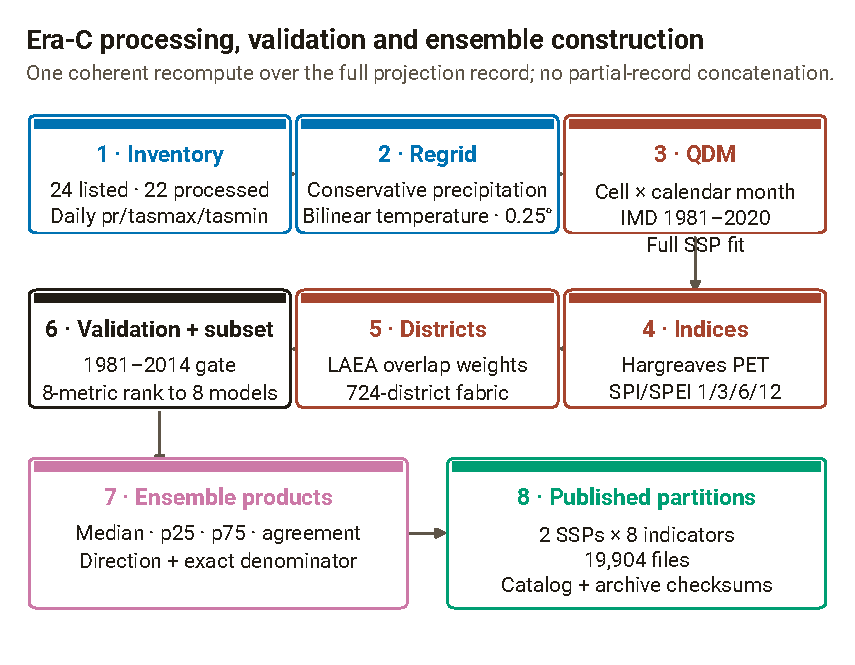
\includegraphics[width=\textwidth]{fig02_projection_pipeline.pdf}
\caption{Era-C processing and ensemble construction. Daily CMIP6 fields from 24 listed models pass an inventory gate; 22 models supply precipitation and temperature. The common chain comprises regridding, quantile delta mapping against IMD, Hargreaves--Samani PET, SPI/SPEI calculation, district aggregation, historical-corrected validation and subset selection. The published eight-model ensemble includes median, spread, model agreement and per-model member series. Historical-corrected, scenario and comparison windows are kept separate.}
\end{figure}

\subsection*{Data engineering and publication}
Era-B values are published as ten wide CSV matrices and as long-format Parquet files with dictionary-encoded identifiers, integer year and month fields, float32 values, zstd compression and deterministic source checksums. Era A is partitioned by variable and year. Era C is partitioned by scenario, statistic, variable and year. The cross-validation product contains matched overlap, per-district and monthly tables. Exact paths are listed in \path{catalog.json}; the browser never discovers files by HTTP globbing.

A monthly era-B refresh runs the existing extraction, indicator and export stages, incrementally reconverts only changed variables, rebuilds the national aggregate and regenerates the catalogue and status artifact. The regression baseline is reviewed and re-blessed explicitly; the refresh command never approves its own data drift. Versioned data bundles are archived at Zenodo\citep{DeshmukhData2026} and served as an immutable snapshot through static HTTP Range requests. DuckDB-WASM runs analytical SQL in a browser Web Worker, with a permanent CSV fallback for the wide matrices.

\section*{Data Records}
The version 2.0.0 dataset is archived at Zenodo under \url{https://doi.org/10.5281/zenodo.24445534}\citep{DeshmukhData2026}. The deposit contains four ZIP bundles, a README and a SHA-256 manifest: era A (20.4~MB), era B (11.4~MB), era C (900.1~MB) and cross-validation (8.2~MB). The immutable public snapshot is \texttt{v2026.09} at \url{https://data.ankitdeshmukh.com/v2026.09/}. Table 5 lists the deposited archives and the companion artifacts available in the repository and public snapshot.

\begin{table}[t]
\caption{Deposited archives and companion artifacts.}
\small
\begin{tabularx}{\textwidth}{@{}>{\RaggedRight\arraybackslash}p{0.36\textwidth}>{\RaggedRight\arraybackslash}p{0.18\textwidth}>{\RaggedRight\arraybackslash}X@{}}
\toprule
File or pattern & Format & Contents \\
\midrule
\path{die-v2.0.0-era-a-atlas.zip} & ZIP/Parquet & 375 partitions; SPEI-1/4/12, 1901--2025; 3,220,872 district-month rows \\
\path{die-v2.0.0-era-b-gridded.zip} & ZIP/CSV/Parquet & Ten wide matrices and ten long Parquet files, 1981-01--2026-09 \\
\path{die-v2.0.0-era-c-projections.zip} & ZIP/Parquet & 19,904 scenario--statistic--variable--year partitions, 2015--2100 \\
\path{die-v2.0.0-cross-validation.zip} & ZIP/Parquet & Overlap, per-district and monthly era-A--era-B tables, 1981--2014 \\
\path{README.md} and \path{SHA256SUMS.txt} & Markdown/text & Archive inventory, schema, licences and checksums \\
\path{data/metadata.json}, \path{catalog.json} & JSON & Indicator contract, exact paths, provenance and era metadata \\
\path{parquet/_national_monthly.parquet} & Parquet & Area-weighted national monthly series with valid district counts \\
\path{data/events/baseline_1981_2014.json} & JSON & Frozen era-B event baseline used by projection comparisons \\
\path{data/imd_validation.json}, \path{data/reality_checks.json} & JSON & Independent IMD comparison and documented-event checks \\
\path{data/boundaries/*.geojson} & GeoJSON & District, state and national-outline geometries \\
\bottomrule
\end{tabularx}
\end{table}

The core district-month schema is \path{district_id}, \path{year}, \path{month} and \path{value}. Era-C files add scenario, statistic and model-denominator fields through partition paths and metadata; direction-agreement files include an explicit denominator. Monthly value and member partitions cover 720 districts; denominator partitions retain all 724 district rows, with zero denominators for the four districts lacking monthly series. The cross-validation overlap table contains \path{variable}, \path{district_id}, \path{date}, era-A and era-B values, their difference, drought flags, class labels and event-match indicators. The per-district table contains sample size, coverage, correlation, bias, root-mean-square difference, seam standard deviation and categorical agreement measures. Table 6 defines the principal fields.

\begin{table}[t]
\caption{Principal data fields and semantics.}
\small
\begin{tabularx}{\textwidth}{@{}>{\RaggedRight\arraybackslash}p{0.20\textwidth}>{\RaggedRight\arraybackslash}p{0.15\textwidth}>{\RaggedRight\arraybackslash}X@{}}
\toprule
Field & Type or values & Meaning \\
\midrule
\path{district_id} & dictionary string & Stable state-prefixed district slug used across all eras \\
\path{year}, \path{month} & int16, int8 & Calendar year and month (1--12) \\
\path{value} & float32 & Indicator value: z for SPI/SPEI, percent for SMA, 0--100 for VCI, model fraction for agreement statistics \\
\path{variable} & dictionary string & Indicator identifier such as \path{spi_03}, \path{spei_12}, \path{sma} or \path{vci} \\
\path{scenario} & partition key & \path{ssp245} or \path{ssp585} for era C \\
\path{stat} & partition key & Median, p25, p75, agreement, direction, denominator or member statistic \\
\path{n_districts} & int16 & Number of finite districts contributing to a national monthly aggregate \\
\path{n_models} & int16 & Exact model denominator for an ensemble statistic; zero where no monthly series exists \\
\path{date} & string YYYY-MM & Calendar date in cross-validation tables \\
\path{r}, \path{bias}, \path{rmsd} & double & Per-district overlap correlation, mean difference and root-mean-square difference \\
\path{sd_diff} & double & Population standard deviation of era-B minus era-A differences over 1981--2014 \\
\path{flag_a}, \path{flag_b} & class string & Drought-state flags for the two eras \\
\path{class_match}, \path{class_near} & boolean & Exact and within-one-class categorical agreement \\
\bottomrule
\end{tabularx}
\end{table}

Missing observations are absent rows in Parquet and empty cells in CSV. Zero is a valid measurement and is never used as a missing-value sentinel. Every national aggregate carries the number of valid districts. Metadata record the reference period, source collections, processing versions, quality flags, known limitations, licences and retrieval dates. Companion files not listed as separate Zenodo archive entries remain available in the software repository and public snapshot.

\section*{Data Overview}
Figure 3 summarises the record windows and era-B indicator availability. The coverage display is descriptive of file contents only; it does not present drought results.

\begin{figure}[t]
\centering
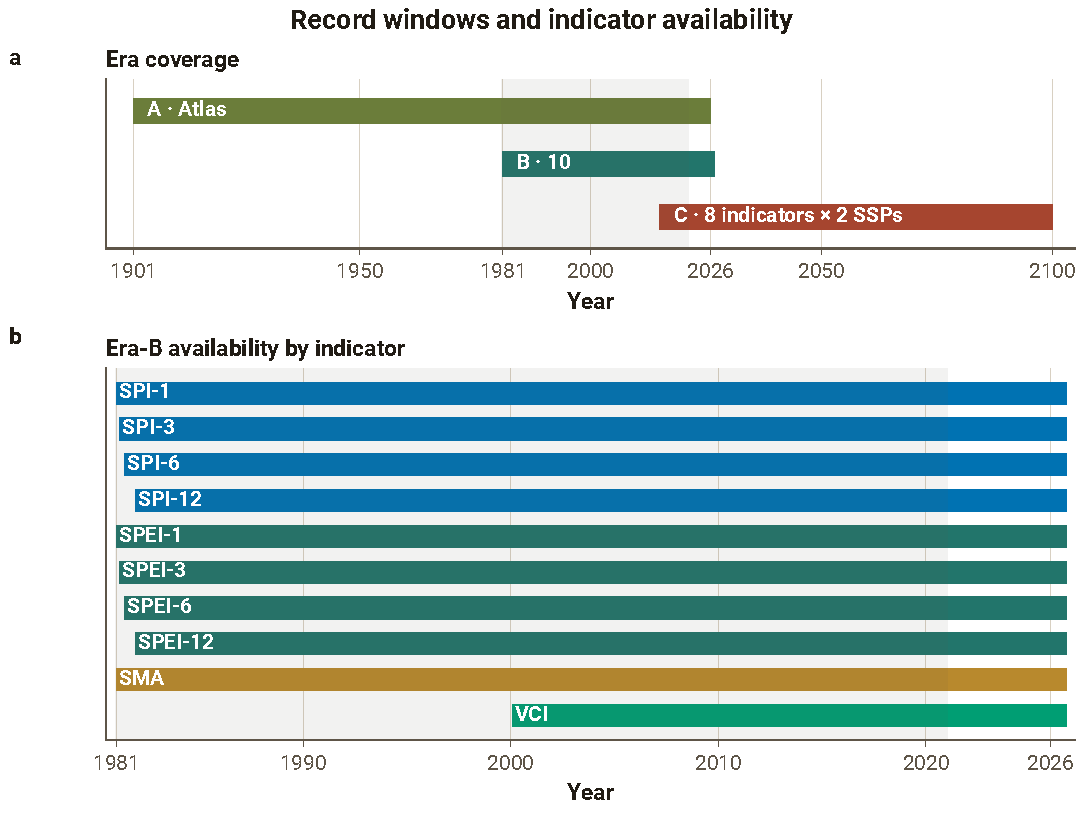
\includegraphics[width=\textwidth]{fig03_coverage.pdf}
\caption{Record windows and indicator availability. (a) Era windows: Atlas reconstruction (1901--2025), gridded multi-source indicators (1981-01--2026-09) and CMIP6 projections (2015--2100). (b) Availability of the ten era-B indicators; the shaded band marks the 1981--2020 standardisation reference, and multi-month windows begin after their accumulation warm-up. VCI begins with the MODIS record in February 2000.}
\end{figure}

\section*{Technical Validation}

\subsection*{Pipeline, fit and round-trip checks}
The era-B pipeline self-test executes 82 deterministic assertions on a synthetic world with an injected drought, vegetation gaps and a missing soil-moisture month. The shipped-data regression harness checks 735 baseline values, including source checksums, catalogue entries, CSV--Parquet round trips, regional anchors, the national aggregate, reality checks and IMD benchmark values. The converter verifies random source cells and checks absence patterns; the national aggregate was independently recomputed row by row. The Atlas ingestion includes source-cell round trips, and the CMIP6 pipeline includes synthetic end-to-end tests for regridding, bias correction, PET, index calculation, aggregation, ensemble statistics and export. Executable verification entry points are listed in Code Availability and in the package checklist.

\begin{table}[t]
\caption{Dashboard windows, direct links and supported analyses.}
\small
\begin{tabularx}{\textwidth}{@{}>{\RaggedRight\arraybackslash}p{0.20\textwidth}>{\RaggedRight\arraybackslash}p{0.34\textwidth}>{\RaggedRight\arraybackslash}X@{}}
\toprule
Window or page & What it shows & Supported analyses \\
\midrule
\href{https://drought.ankitdeshmukh.com/\#overview}{Overview} & Current-month choropleth, affected area, severity, district counts, national series and evolution & Area-weighted drought extent, severity ranking, month-to-month change and animation \\
\href{https://drought.ankitdeshmukh.com/\#historical}{Historical Analysis} & Frequency, duration, severity, recurrence and long-term trends & Seasonal summaries, Mann--Kendall, Sen slope, Hamed--Rao correction and BH-FDR district significance \\
\href{https://drought.ankitdeshmukh.com/\#events}{Drought Events} & Runs-analysis event catalogue and event maps & Onset, termination, duration, peak, cumulative severity, recovery, censoring and definition sensitivity \\
\href{https://drought.ankitdeshmukh.com/\#propagation}{Propagation \& Relationships} & Pairwise lag correlation, confidence bands and relationship maps & Lag $-12$ to $+12$ months, block-bootstrap intervals, optimal lag and indicator-pair comparison \\
\href{https://drought.ankitdeshmukh.com/\#crossval}{Cross-validation} & Era-A--era-B agreement, discrepancy maps and monthly agreement & Correlation, bias, RMSD, drought-state and class agreement, and seam uncertainty \\
\href{https://drought.ankitdeshmukh.com/\#/district/rajasthan-jodhpur}{District profile} & One-district headline, ten-indicator strip, trend, events and era context & District-month interrogation, trend and event forensics, and labelled cross-era context \\
\href{https://drought.ankitdeshmukh.com/\#projections}{Future Projections} & Scenario, statistic and time-window controls with ensemble band, map and model context & Median, p25--p75 spread, moderate/severe agreement, model comparison, SPI--SPEI divergence and future events \\
\href{https://drought.ankitdeshmukh.com/\#summary}{Drought to 2100} & Direction-of-change map, national summary and per-state table & Drought-month share, event duration and severity deltas; share of models drier than their own base \\
\href{https://drought.ankitdeshmukh.com/\#atlas}{Atlas} & 1901--2025 SPEI scrubber, class shares and historical anchors & Reconstruction climatology, drought-class frequency and historical-event anchoring \\
\href{https://drought.ankitdeshmukh.com/\#engine}{Engine Lab} & Catalogue, SQL editor, query results, timing and byte counter & Read-only Parquet SQL, custom district/month queries and CSV export \\
\href{https://drought.ankitdeshmukh.com/\#data}{Documentation} & Methods, governance, licences, reality checks, status, downloads and SQL guide & Provenance inspection, reproduction instructions, data access and query reference \\
\href{https://drought.ankitdeshmukh.com/tour.html}{Guided tour} & Standalone onboarding and era primer & Navigation, interpretation guardrails and first-use orientation \\
\bottomrule
\end{tabularx}
\end{table}

The indicator fit report records the number of fitted, Gringorten-fallback and calibration-fallback series. Base transformed values are required to remain within the declared mean and standard-deviation gates, and a minimum of 20 base years is enforced. The released \path{data-pipeline/verify_paper_claims.py} script reproduces six methodological experiments, including L-moment parameter recovery, the small-sample maximum-likelihood wet bias, tie handling in the Gringorten transform, classification continuity, area-weighting accuracy and the Benjamini--Hochberg demonstration. In 300 synthetic log-logistic replications at $n=40$, the mean transformed base value was $+0.79$ under maximum likelihood and $+0.01$ under L-moments; this is a property of the tested simulation setting, not a general theorem. On the current SPI-3 record, 415 districts are significant before multiple-testing control and 354 after Benjamini--Hochberg control, superseding the version 1.0.0 values of 382 and 324.

\subsection*{Boundary and documented-event checks}
The served national area is 3,266,386~km$^2$, compared with India's published 3,287,263~km$^2$. The unsimplified source fabric totals 3,266,465~km$^2$ for 726 district features and 3,266,382~km$^2$ after removing two exact duplicates. Generalisation therefore accounts for only a few square kilometres; the remaining shortfall is a property of the community boundary source. Median district-area error between the served and unsimplified geometries is 0.034\%, with a 95th percentile of 0.15\%.

Three documented-event checks are re-derived from the shipped matrices. Every Rajasthan district is at or below $-1.00$ SPI-3 in July, August and September 2002, with area-weighted means of $-2.55$, $-2.68$ and $-2.54$. All-India SPI-3 is at or below $-1.00$ in 4 of 547 available months: July 1987 and July--September 2002; these form one qualifying three-month event under the frozen rule. For Marathwada in 2015--2016, mean SPI-3 is $-0.97$ in September 2015, mean VCI is 13.5 in November 2015 and 8.4 in January 2016. The checks demonstrate temporal and geographic consistency; they are not an independent accuracy certification. Applying the current default rules to the full SPI-3 matrix yields 8,044 events, of which 61 are right-censored at the record end.

\subsection*{Independent IMD benchmark}
The era-B record was compared with an independently processed IMD archive over 1981--2025 (Table 8; Fig. 4). IMD rainfall is available at 0.25$^\circ$ and temperature at 1.0$^\circ$. The benchmark uses the same district fabric, indicator code, 1981--2020 reference period and missing-data policy. SPI is the primary like-for-like comparison because rainfall inputs and estimators are shared. SPEI includes a PET-method difference because the benchmark uses Hargreaves--Samani PET from IMD temperature while era B uses ERA5-Land PET. The computed benchmark retains its full 1981--2025 overlap; it is not relabelled as the 1981--2014 window used for Atlas and climate-model comparisons.

Median district correlations range from 0.604 to 0.714, and area-weighted bias ranges from $-0.038$ to $+0.002$ z. Drought-state agreement is 82.2--86.9\%. At $q=0.05$, era B identifies more significant annual SPI-3 trends than IMD (324 versus 155 districts), but slope signs agree for 89.3\% of districts significant in both records. This difference is reported rather than smoothed: smoother gridded inputs and different PET formulations affect detection power. The 1.0$^\circ$ temperature grid also limits the spatial detail of benchmark SPEI.

\begin{table}[t]
\caption{Independent IMD benchmark, 1981--2025. Bias is area-weighted IMD minus era B.}
\small
\begin{tabularx}{\textwidth}{@{}>{\RaggedRight\arraybackslash}lrrrrrr@{}}
\toprule
Indicator & Districts & Pairs & Median $r$ & Bias (z) & State agreement & Exact class \\
\midrule
SPI-1 & 719 & 388,260 & 0.675 & +0.002 & 86.9\% & 36.5\% \\
SPI-3 & 719 & 386,822 & 0.659 & $-0.018$ & 83.9\% & 33.7\% \\
SPI-6 & 719 & 384,665 & 0.643 & $-0.027$ & 83.4\% & 33.0\% \\
SPI-12 & 719 & 380,351 & 0.604 & $-0.030$ & 82.2\% & 31.7\% \\
SPEI-3 & 714 & 384,068 & 0.714 & $-0.028$ & 84.9\% & 35.6\% \\
SPEI-12 & 714 & 377,624 & 0.647 & $-0.038$ & 84.3\% & 32.7\% \\
\bottomrule
\end{tabularx}
\end{table}

\begin{figure}[t]
\centering
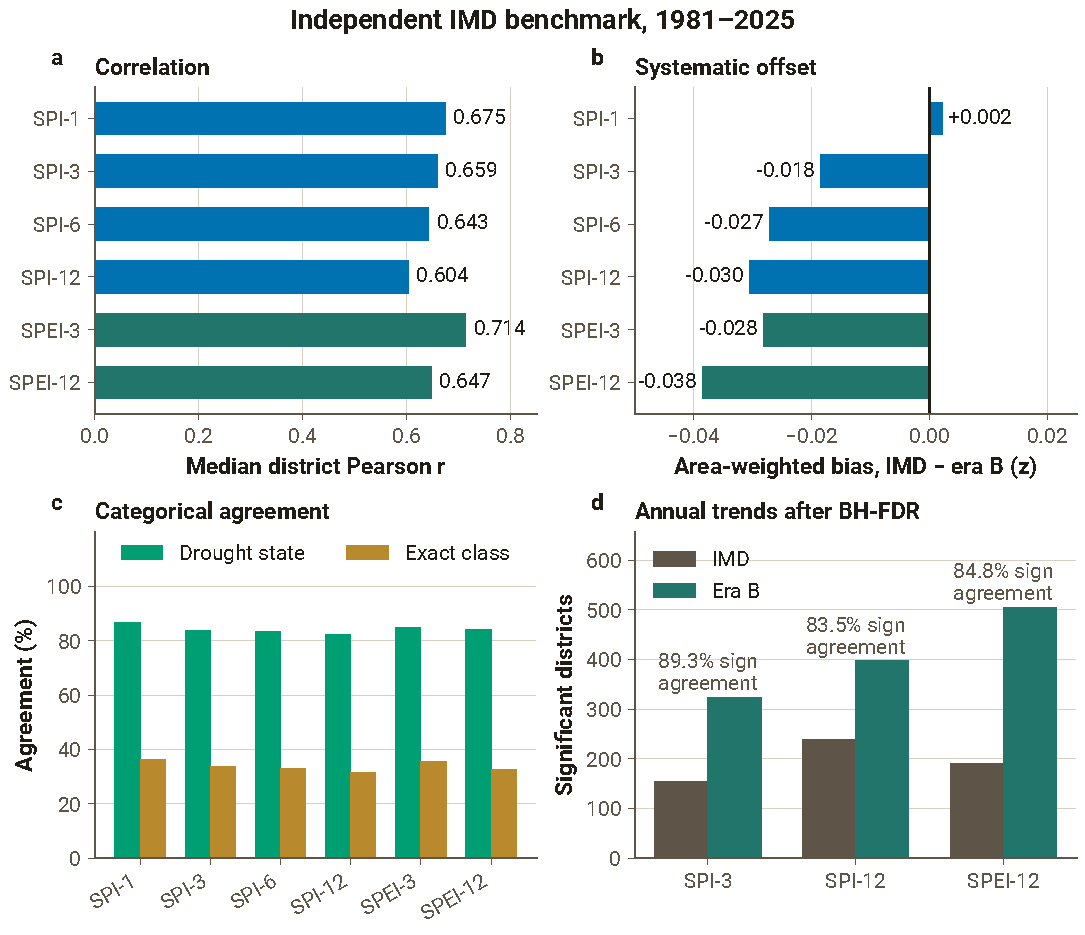
\includegraphics[width=\textwidth]{fig04_imd_benchmark.pdf}
\caption{Independent IMD benchmark, 1981--2025, with a common 1981--2020 standardisation base. (a) Median district Pearson correlation for 719 SPI and 714 SPEI districts. (b) Area-weighted mean difference, IMD minus era B. (c) Agreement on drought state at the $-1.00$ truncation and on exact nine-class category. (d) Districts with significant annual trends after Benjamini--Hochberg control at $q=0.05$; annotations show slope-sign agreement among districts significant in both records. SPEI includes a PET-method difference between ERA5-Land and Hargreaves--Samani. Values are point estimates from the committed comparison artifact; no confidence intervals are implied.}
\end{figure}

\subsection*{Era-A and era-B overlap}
The reconstruction and gridded eras are compared only over their common 1981--2014 window (Table 9; Fig. 5). SPEI-1 and SPEI-12 are the shared timescales. The comparison contains 718 districts; the six island districts absent from the Atlas remain missing. Median district correlation is 0.717 for SPEI-1 and 0.667 for SPEI-12. Area-weighted bias is $+0.044$ and $+0.008$ z, respectively, and drought-state agreement is 83.6\% and 82.9\%. Within-one-class agreement is 78.1\% and 75.8\%. The per-district standard deviation of the era-B minus era-A difference has a median of 0.78 z for SPEI-12. This seam statistic measures historical disagreement and is not a projection error bar.

\begin{table}[t]
\caption{Era-A--era-B overlap comparison, 1981--2014.}
\small
\begin{tabularx}{\textwidth}{@{}>{\RaggedRight\arraybackslash}lrrrrrr@{}}
\toprule
Variable & Districts & Matched months & Median $r$ & Area bias (z) & State agreement & Exact class \\
\midrule
SPEI-1 & 718 & 292,925 & 0.717 & +0.044 & 83.6\% & 36.4\% \\
SPEI-12 & 718 & 285,046 & 0.667 & +0.008 & 82.9\% & 34.5\% \\
\bottomrule
\end{tabularx}
\end{table}

\begin{figure}[t]
\centering
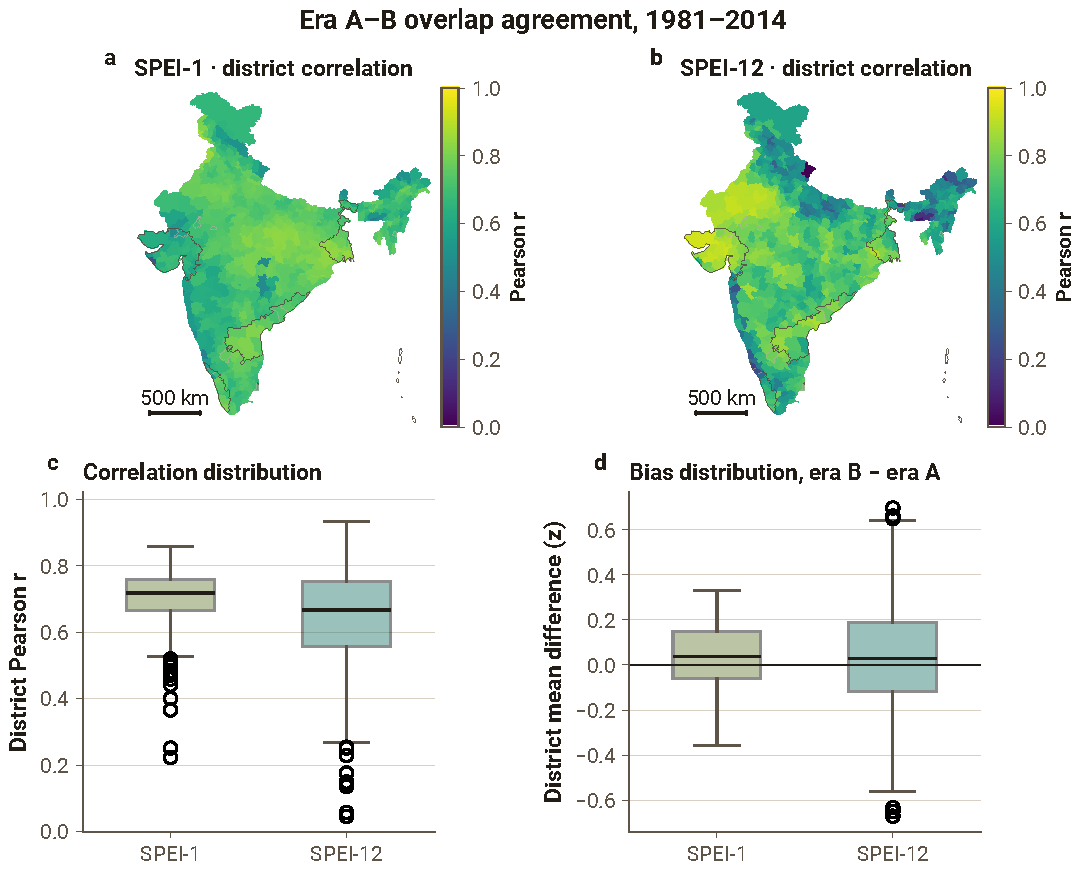
\includegraphics[width=\textwidth]{fig05_atlas_overlap.pdf}
\caption{Era-A--era-B overlap agreement, 1981--2014. (a,b) District correlations for SPEI-1 and SPEI-12; grey denotes districts absent from the Atlas grid. (c,d) Distributions of district correlation and district-mean difference, era B minus era A. Boxes show the interquartile range and median, whiskers extend to 1.5 times the interquartile range, and points are values outside the whiskers. The maps use a common 0--1 correlation scale. Area-weighted bias and agreement are reported in Table 9.}
\end{figure}

\subsection*{CMIP6 release gates}
The historical-corrected gate evaluates 22 models over 1981--2014; the SSP gate evaluates the committed eight-model subset over the 2015--2020 observed overlap and checks historical--scenario continuity (Table 10; Fig. 6). National distribution-shape ratios for the eight indicators lie between 1.018 and 1.056, inside the declared 0.70--1.40 range. Across 1,360 region--season cells, historical consistency has no breaches, drought-event statistics have 41 breaches (15.1\%, below the 25\% limit) and drought-tail statistics have 28 breaches (2.1\%, below the 25\% limit). SSP distribution-shape breaches are 173 of 1,360 (12.7\%) for SSP2-4.5 and 165 of 1,360 (12.1\%) for SSP5-8.5, both below the 20\% limit. The seam gate reports zero breaches among 24 model--variable cells for each scenario.

The gate design changed after two documented remediation rounds. Weather reproduction over the six-year SSP overlap is reported but not gated because free-running simulations do not reproduce the timing of individual observed events. The reported-only overlap diagnostics show drought-statistic breaches of 52.2\% and 57.4\% and tail breaches of 30.2\% and 29.6\% for SSP2-4.5 and SSP5-8.5, respectively. The release gate therefore tests distribution shape, drought statistics over the longer historical-corrected window, tail behaviour and seam continuity. This distinction is retained in the committed reports.

\begin{table}[t]
\caption{CMIP6 release-gate results from committed validation snapshots.}
\small
\begin{tabularx}{\textwidth}{@{}>{\RaggedRight\arraybackslash}p{0.21\textwidth}>{\RaggedRight\arraybackslash}p{0.19\textwidth}rr>{\RaggedRight\arraybackslash}p{0.10\textwidth}>{\RaggedRight\arraybackslash}X@{}}
\toprule
Gate & Window/basis & Breaches & Cells & Limit & Result \\
\midrule
Historical consistency & 1981--2014, 22 models & 0 & 1,360 & 20\% & Pass \\
Historical drought statistics & 1981--2014, 22 models & 41 & 272 & 25\% & Pass \\
Historical tails & 1981--2014, 22 models & 28 & 1,360 & 25\% & Pass \\
SSP2-4.5 shape & 2015--2020 overlap, 8 models & 173 & 1,360 & 20\% & Pass \\
SSP5-8.5 shape & 2015--2020 overlap, 8 models & 165 & 1,360 & 20\% & Pass \\
SSP2-4.5 seam & Historical tail/SSP head & 0 & 24 & Declared tolerances & Pass \\
SSP5-8.5 seam & Historical tail/SSP head & 0 & 24 & Declared tolerances & Pass \\
\bottomrule
\end{tabularx}
\end{table}

\begin{figure}[t]
\centering
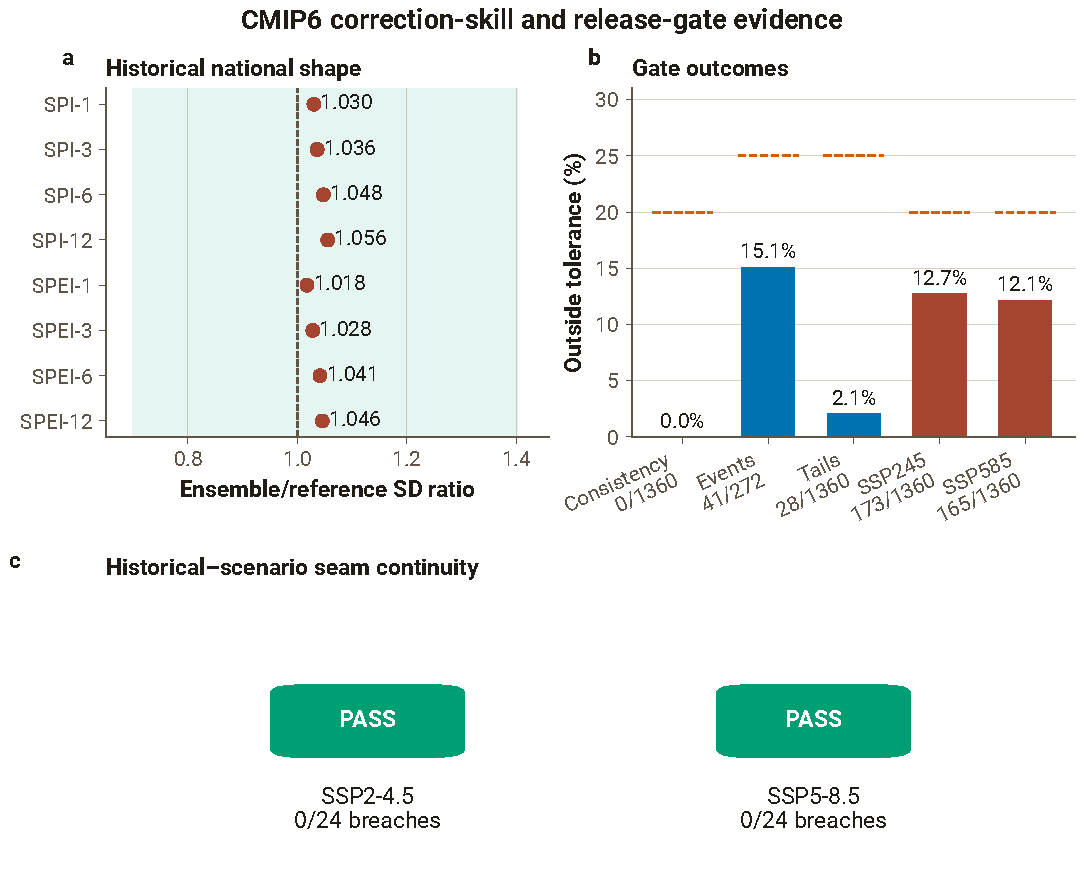
\includegraphics[width=\textwidth]{fig06_gcm_validation.pdf}
\caption{CMIP6 correction-skill and release-gate evidence on a pooled multi-model basis. (a) National ensemble-to-reference standard-deviation ratios for historical-corrected simulations; the shaded region is the declared 0.70--1.40 gate range. (b) Region--season cells outside tolerance, with failure thresholds shown as dashed lines: 20\% for consistency and shape, and 25\% for historical drought statistics and tails. Counts are printed below each category. (c) Historical--scenario seam breaches for 24 model--variable cells in each scenario. Gate values are taken from the committed validation snapshots.}
\end{figure}

\subsection*{Published-claim verification}
The propagation statistic is reproduced from the national monthly series: SPI-3 and SPEI-3 have Pearson $r=0.8716$ over 547 paired months, with a 95\% moving-block bootstrap interval of $[0.8356,0.8999]$ (1,000 resamples, block length 8, seed 20261103). The figure-reproduction command regenerates the coverage, historical and propagation artifacts and the reality-check table reference. Input and output checksums make record--manuscript drift visible. The publication-figure generator additionally records every plotted value, source checksum and output checksum, and rejects plotted text below 10~pt. The two method-flow schematics are authored as Mermaid text and rendered with Pele, so node sizes follow their labels; they print at 8.8 and 9.1~pt at the published width.

\section*{Usage Notes}
The application is available at \url{https://drought.ankitdeshmukh.com/}. Record, Atlas and Projections are separate products; analytical lenses sit beneath the active product. District profiles, map states and panel controls can be shared through encoded permalinks. Exported CSV and text files include citation, licence, generation date and methodology headers. The Engine Lab accepts validated SQL over the published Parquet store and reports row counts, execution time and bytes read. Table 7 provides direct links and a concise description of the analyses supported by every window. Figure 7 summarises the purpose, products, technology and research positioning of the platform: an interactive, fully client-side geospatial platform for exploring drought indicators across Indian districts, built for historical analysis and research communication---not operational monitoring. Figure 8 shows the Record analyses, Figure 9 shows event forensics and indicator relationships, Figure 10 shows the Atlas and projection products, and Figure 11 shows district access and the query interface. The screenshots use the recorded July 2002 default observation and the default projection settings.

\begin{figure}[t]
\centering
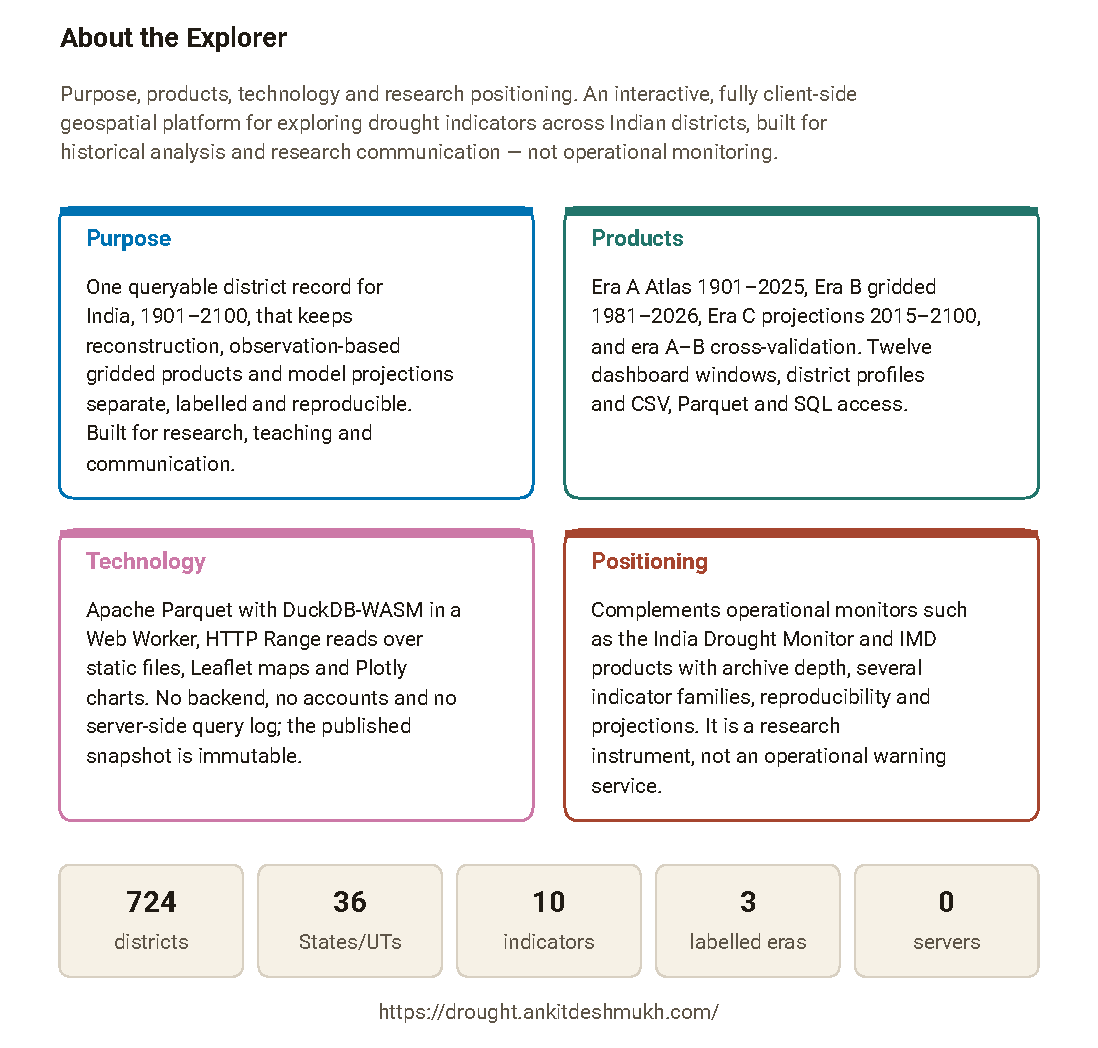
\includegraphics[width=\textwidth]{fig07_about.pdf}
\caption{About the Explorer. Purpose, products, technology and research positioning of the published interface: an interactive, fully client-side geospatial platform for exploring drought indicators across Indian districts, built for historical analysis and research communication---not operational monitoring. The cards summarise the purpose, the three labelled era products with the cross-validation layer, the client-side technology stack, and the positioning relative to operational monitors; the strip reports the district fabric, indicator families and server footprint.}
\end{figure}

\begin{figure}[t]
\centering
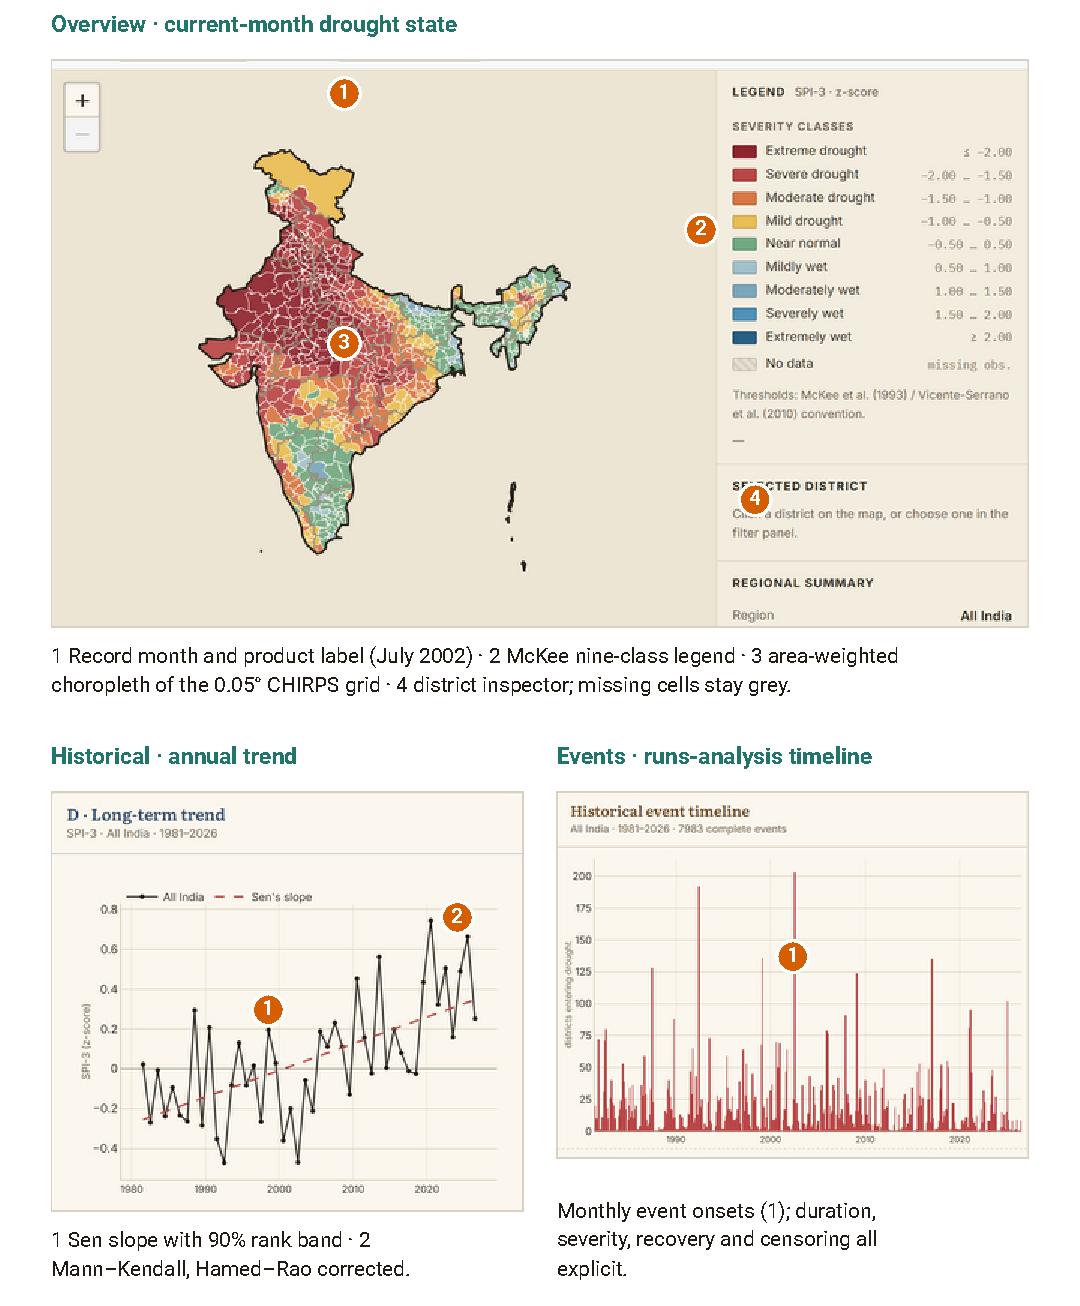
\includegraphics[width=\textwidth]{fig08_record_analyses.pdf}
\caption{Record analyses: current state, long-term trend and event catalogue. (Top) Overview workspace at the recorded July 2002 default state: (1) record month and product label, (2) McKee nine-class severity legend, (3) area-weighted district choropleth of the 0.05$^\circ$ CHIRPS grid, and (4) the district inspector; missing cells stay grey and are never imputed. (Bottom left) Historical Analysis annual trend with the Sen slope and Mann--Kendall statistics under the Hamed--Rao correction. (Bottom right) Drought Events monthly onsets from the runs-analysis catalogue. Screenshots were captured from the live site on 25 November 2026.}
\end{figure}

\begin{figure}[t]
\centering
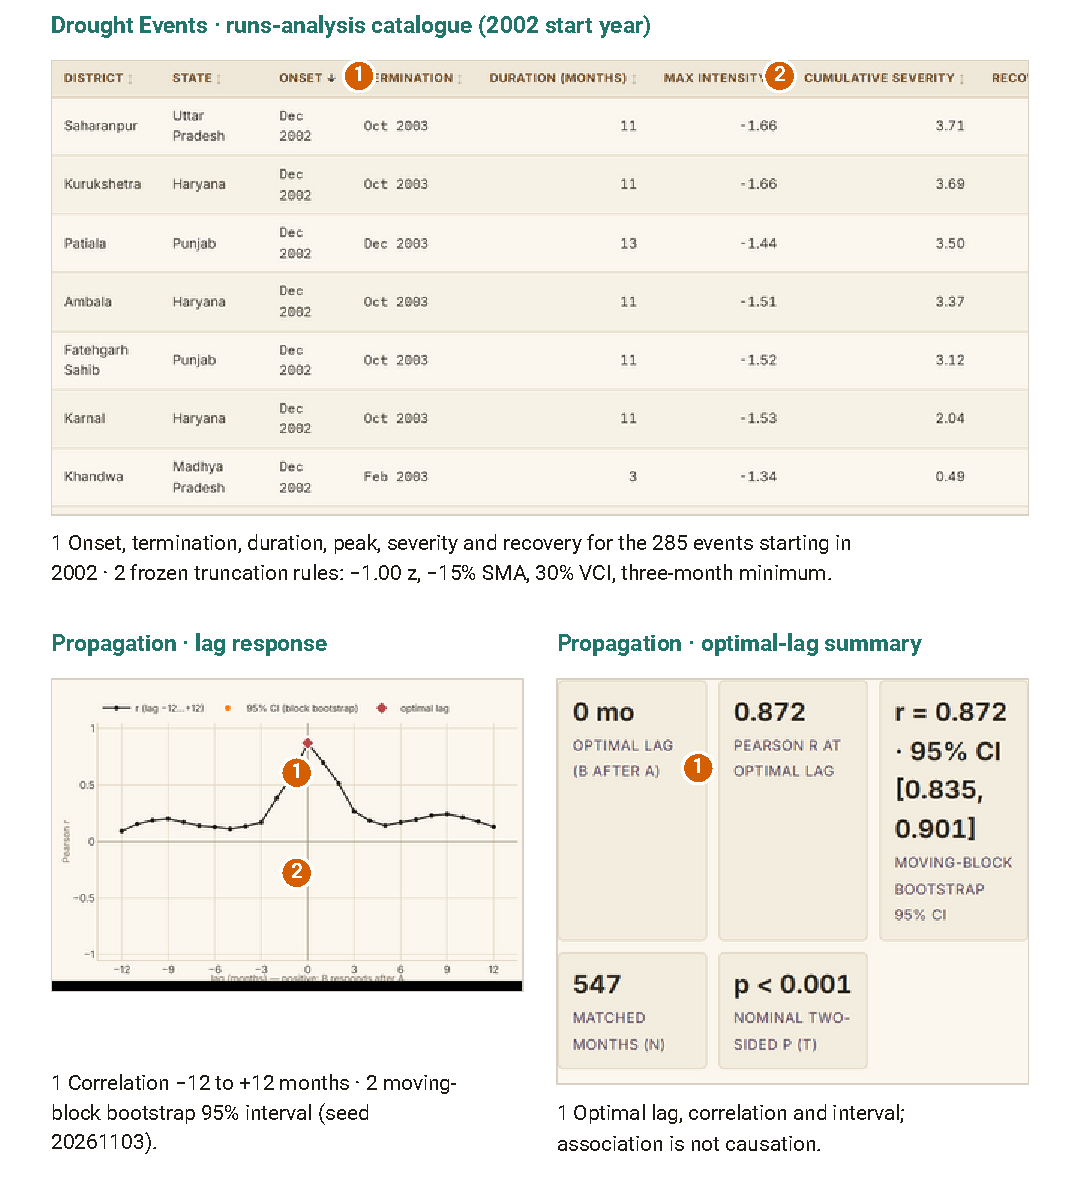
\includegraphics[width=\textwidth]{fig09_events_propagation.pdf}
\caption{Event forensics and indicator relationships. (Top) Drought Events catalogue filtered to the 285 events starting in 2002, with onset, termination, duration, peak intensity, cumulative severity and recovery; truncation is the upper bound of the moderate class ($-1.00$~z, $-15\%$ SMA, 30\% VCI) with a three-month minimum duration, and censored events are flagged. (Bottom) Propagation \& Relationships: Pearson correlation from $-12$ to $+12$ months with the moving-block bootstrap 95\% interval (1,000 resamples, seed 20261103) and the optimal-lag summary for the selected pair; the panel states in place that association is not causation.}
\end{figure}

\begin{figure}[t]
\centering
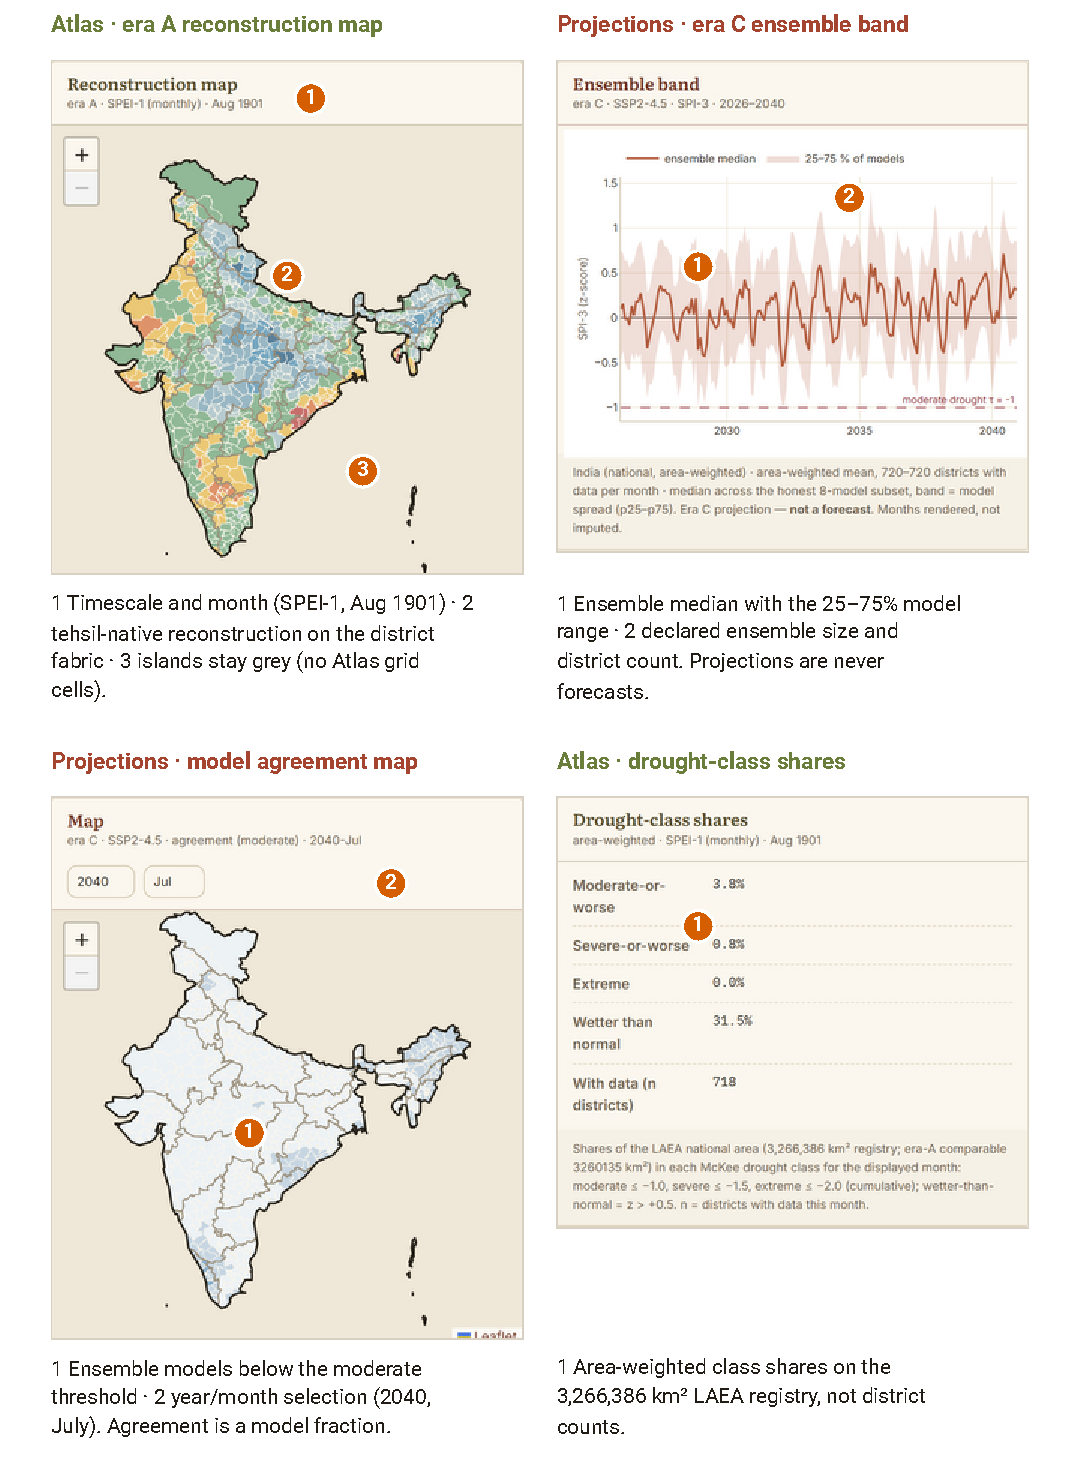
\includegraphics[width=\textwidth]{fig10_atlas_projections.pdf}
\caption{Reconstruction and projection products. (Top left) Atlas era-A reconstruction map (SPEI-1, August 1901) served on the district fabric, with 718 districts carrying a value at that month and island units grey. (Top right) Era-C ensemble band for SSP2-4.5 SPI-3, 2026--2040, showing the median, the 25--75\% model range and the declared ensemble size. (Bottom left) District-level model agreement map for the moderate threshold at July 2040. (Bottom right) Area-weighted drought-class shares on the 3,266,386~km$^2$ LAEA registry. Era A and era C are separate labelled products and are never spliced into the era-B record. Screenshots were captured from the live site on 25 November 2026.}
\end{figure}

\begin{figure}[t]
\centering
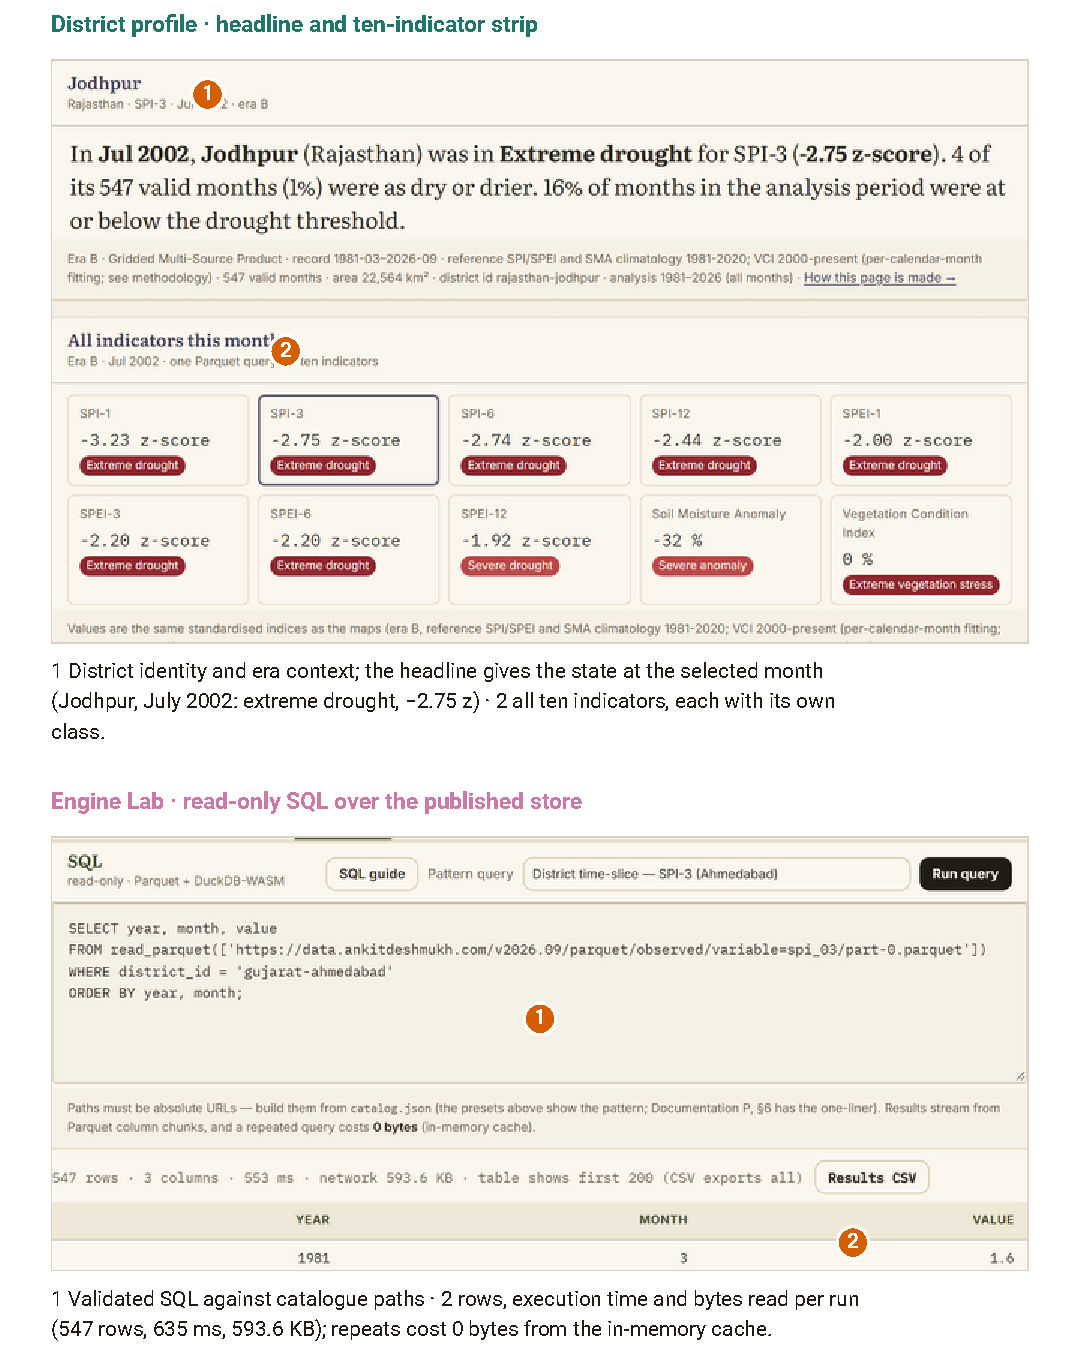
\includegraphics[width=\textwidth]{fig11_access_reuse.pdf}
\caption{District access and reproducible query. (Top) District-profile headline for Jodhpur at July 2002 (extreme drought, $-2.75$~z SPI-3), with era, record coverage and analysis window. (Middle) The ten-indicator strip at the same district and month, each indicator with its own class. (Bottom) Engine Lab running a validated pattern query over the published Parquet store; every run reports row count, execution time and bytes read, and repeated queries cost 0 bytes from the in-memory cache.}
\end{figure}

The dataset can also be used without the application. The wide CSV matrices are convenient for spreadsheet and statistical workflows. Long-format Parquet files support columnar analysis in Python, R or DuckDB, and the catalogue supplies exact paths for HTTP Range reads. The core district-month query pattern is:

\begin{verbatim}
SELECT district_id, year, month, value
FROM read_parquet('data/parquet/observed/variable=spi_03/part-0.parquet')
WHERE district_id = 'rajasthan-jodhpur'
ORDER BY year, month;
\end{verbatim}

A national monthly query uses the pre-aggregate and retains its denominator:

\begin{verbatim}
SELECT year, month, value, n_districts
FROM read_parquet('data/parquet/_national_monthly.parquet')
WHERE variable = 'spi_03'
ORDER BY year, month;
\end{verbatim}

An era-C ensemble query must keep scenario and statistic explicit:

\begin{verbatim}
SELECT district_id, year, month, value, n_models
FROM read_parquet('data/parquet/projections/scenario=ssp245/
                  stat=agreement_moderate/variable=spi_03/year=2090/
                  part-0.parquet')
ORDER BY district_id, month;
\end{verbatim}

Analysts should retain era, source and reference-period fields when combining results, report the valid sample size for every statistic and preserve missing values as missing. Era A, era B and era C should be compared through the published overlap products rather than concatenated. Agreement statistics are model fractions, not probabilities, and direction agreement is a count over a declared window.

Several limitations constrain interpretation. District values inherit source-grid and aggregation uncertainty; small districts and buffered island units have reduced effective support. The boundary fabric has a 2011-era lineage and does not represent later reorganisations. CHIRPS, ERA5-Land and MODIS retain their documented biases. Era-B SPEI uses reanalysis PET, whereas era-C SPEI uses Hargreaves--Samani PET; the methods share index construction but not PET physics. VCI's release-dependent baseline can shift when the MODIS record is extended. Event and trend results depend on the declared thresholds and sample rules, and spatial dependence limits the interpretation of district-level significance.

The projection ensemble contains one realisation from each of eight selected models. It does not represent the full CMIP6 structural uncertainty or internal variability, and selection on historical skill does not guarantee future skill. Ensemble spread and agreement must be inspected together. Bias correction preserves the model's relative change signal by construction but cannot remove uncertainties absent from the reference. Correlation, lagged association and propagation displays do not establish causation, and no streamflow, groundwater, crop-loss or health claims should be inferred from these indicators alone. The resource is a research and teaching instrument, not an operational warning service.

\section*{Data Availability}
The version 2.0.0 dataset is available at \url{https://doi.org/10.5281/zenodo.24445534}\citep{DeshmukhData2026} under CC BY 4.0. It includes the era-A, era-B, era-C and cross-validation ZIP bundles, a README and SHA-256 manifest. The immutable public snapshot is \url{https://data.ankitdeshmukh.com/v2026.09/}; exact file paths are in \path{data/parquet/catalog.json}. The live application is \url{https://drought.ankitdeshmukh.com/}. Original source products retain their own terms: CHIRPS public domain, ERA5-Land Copernicus licence, MODIS open data, Atlas CC BY 4.0, CMIP6 model-specific terms and IMD terms. Raw IMD and CMIP6 inputs are not redistributed in the DIE archive.

\section*{Code Availability}
The processing pipelines, browser application, configuration files, tests and publication-figure generator are available at \url{https://github.com/anixn/drought-intelligence-explorer} and archived as version 2.0.0 under the MIT licence at \url{https://doi.org/10.5281/zenodo.24444860}\citep{DeshmukhSoftware2026}.

The main entry points are \path{data-pipeline/run.py}, \path{data-pipeline/selftest.py}, \path{data-pipeline/verify_paper_claims.py}, \path{atlas-pipeline/}, \path{gcm-pipeline/} and \path{validation-studies/}. Publication and verification scripts include \path{scripts/convert_to_parquet.py}, \path{scripts/regression_check.py}, \path{scripts/verify_reality_checks.py}, \path{scripts/reproduce_figures.py}, \path{manuscript/scientific-data/make_figures.py}, \path{manuscript/scientific-data/render_schematics.py} and \path{manuscript/scientific-data/check_manuscript.py}. Scientific and engineering parameters are held in versioned YAML or JSON configuration files. No proprietary service is required to inspect the deposited data or run the offline tests; re-extraction from Google Earth Engine or re-download of CMIP6 requires the corresponding public service credentials and data access.

\begin{thebibliography}{34}
\small
\bibitem{WilhiteGlantz1985} Wilhite, D. A. \& Glantz, M. H. Understanding the drought phenomenon: the role of definitions. \textit{Water Int.} \textbf{10}, 111--120 (1985). \url{https://doi.org/10.1080/02508068508686328}
\bibitem{MishraSingh2010} Mishra, A. K. \& Singh, V. P. A review of drought concepts. \textit{J. Hydrol.} \textbf{391}, 202--216 (2010). \url{https://doi.org/10.1016/j.jhydrol.2010.07.012}
\bibitem{McKee1993} McKee, T. B., Doesken, N. J. \& Kleist, J. The relationship of drought frequency and duration to time scales. In \textit{Proc. 8th Conference on Applied Climatology} 179--184 (American Meteorological Society, 1993).
\bibitem{VicenteSerrano2010} Vicente-Serrano, S. M., Beguer\'{\i}a, S. \& L\'{o}pez-Moreno, J. I. A multiscalar drought index sensitive to global warming: the Standardized Precipitation Evapotranspiration Index. \textit{J. Clim.} \textbf{23}, 1696--1718 (2010). \url{https://doi.org/10.1175/2009JCLI2909.1}
\bibitem{Kogan1995} Kogan, F. N. Application of vegetation index and brightness temperature for drought detection. \textit{Adv. Space Res.} \textbf{15}, 91--100 (1995). \url{https://doi.org/10.1016/0273-1177(95)00079-T}
\bibitem{WMOLincoln2009} World Meteorological Organization. \textit{Inter-regional Workshop on Indices and Early Warning Systems for Drought: Lincoln Declaration on Drought Indices} (WMO, 2009).
\bibitem{Pai2014} Pai, D. S., Sridhar, L., Rajeevan, M., Sreejith, O. P., Satbhai, N. S. \& Mukhopadhyay, B. Development of a new high spatial resolution ($0.25^\circ\times0.25^\circ$) long period (1901--2010) daily gridded rainfall data set over India. \textit{Mausam} \textbf{65}, 1--18 (2014). \url{https://doi.org/10.54302/mausam.v65i1.851}
\bibitem{Srivastava2009} Srivastava, A. K., Rajeevan, M. \& Kshirsagar, S. R. Development of a high resolution daily gridded temperature data set (1969--2005) for the Indian region. \textit{Atmos. Sci. Lett.} \textbf{10}, 249--254 (2009). \url{https://doi.org/10.1002/asl.232}
\bibitem{Chuphal2024} Chuphal, D. S., Kushwaha, A. P., Aadhar, S. \& Mishra, V. Drought Atlas of India, 1901--2020. \textit{Sci. Data} \textbf{11}, 7 (2024). \url{https://doi.org/10.1038/s41597-023-02856-y}
\bibitem{ChuphalData2024} Chuphal, D. S., Kushwaha, A. P., Aadhar, S. \& Mishra, V. \textit{Drought Atlas of India, 1901--2025}, version 2 [Dataset]. Zenodo (2024). \url{https://doi.org/10.5281/zenodo.20368514}
\bibitem{DeshmukhV1Data2026} Deshmukh, A. \textit{Drought Intelligence Explorer: an interactive geospatial platform for drought monitoring and analysis in India}, version 1.0.0 [Computer software and dataset]. Zenodo (2026). \url{https://doi.org/10.5281/zenodo.24113364}
\bibitem{Funk2015} Funk, C. et al. The climate hazards infrared precipitation with stations---a new environmental record for monitoring extremes. \textit{Sci. Data} \textbf{2}, 150066 (2015). \url{https://doi.org/10.1038/sdata.2015.66}
\bibitem{MunozSabater2021} Mu\~{n}oz-Sabater, J. et al. ERA5-Land: a state-of-the-art global reanalysis dataset for land applications. \textit{Earth Syst. Sci. Data} \textbf{13}, 4349--4383 (2021). \url{https://doi.org/10.5194/essd-13-4349-2021}
\bibitem{Didan2015} Didan, K. \textit{MOD13A3 MODIS/Terra Vegetation Indices Monthly L3 Global 1 km SIN Grid V061} [Dataset]. NASA Land Processes Distributed Active Archive Center (2021). \url{https://doi.org/10.5067/MODIS/MOD13A3.061}
\bibitem{Eyring2016} Eyring, V. et al. Overview of the Coupled Model Intercomparison Project Phase 6 (CMIP6) experimental design and organization. \textit{Geosci. Model Dev.} \textbf{9}, 1937--1958 (2016). \url{https://doi.org/10.5194/gmd-9-1937-2016}
\bibitem{ONeill2016} O'Neill, B. C. et al. The Scenario Model Intercomparison Project (ScenarioMIP) for CMIP6. \textit{Geosci. Model Dev.} \textbf{9}, 3461--3482 (2016). \url{https://doi.org/10.5194/gmd-9-3461-2016}
\bibitem{Cannon2015} Cannon, A. J., Sobie, S. R. \& Murdock, T. Q. Bias correction of GCM precipitation by quantile mapping: how well do methods preserve changes in quantiles and extremes? \textit{J. Clim.} \textbf{28}, 6938--6959 (2015). \url{https://doi.org/10.1175/JCLI-D-14-00754.1}
\bibitem{HargreavesSamani1985} Hargreaves, G. H. \& Samani, Z. A. Reference crop evapotranspiration from temperature. \textit{Appl. Eng. Agric.} \textbf{1}, 96--99 (1985). \url{https://doi.org/10.13031/2013.26773}
\bibitem{DeshmukhSoftware2026} Deshmukh, A. \textit{Drought Intelligence Explorer: a multi-era district drought record and analytics platform for India}, version 2.0.0 [Computer software]. Zenodo (2026). \url{https://doi.org/10.5281/zenodo.24444860}
\bibitem{DeshmukhData2026} Deshmukh, A. \textit{Drought Intelligence Explorer v2.0.0---district drought record for India (1901--2100)}, version 2.0.0 [Dataset]. Zenodo (2026). \url{https://doi.org/10.5281/zenodo.24445534}
\bibitem{uditIndiaMaps} udit-001. \textit{india-maps-data} [GitHub repository]. \url{https://github.com/udit-001/india-maps-data} (accessed 24 November 2026).
\bibitem{Gorelick2017} Gorelick, N. et al. Google Earth Engine: planetary-scale geospatial analysis for everyone. \textit{Remote Sens. Environ.} \textbf{202}, 18--27 (2017). \url{https://doi.org/10.1016/j.rse.2017.06.031}
\bibitem{Hersbach2020} Hersbach, H. et al. The ERA5 global reanalysis. \textit{Q. J. R. Meteorol. Soc.} \textbf{146}, 1999--2049 (2020). \url{https://doi.org/10.1002/qj.3803}
\bibitem{Begueria2014} Beguer\'{\i}a, S., Vicente-Serrano, S. M., Reig, F. \& Latorre, B. Standardized precipitation evapotranspiration index (SPEI) revisited: parameter fitting, evapotranspiration models, tools, datasets and drought monitoring. \textit{Int. J. Climatol.} \textbf{34}, 3001--3023 (2014). \url{https://doi.org/10.1002/joc.3887}
\bibitem{Hosking1990} Hosking, J. R. M. L-moments: analysis and estimation of distributions using linear combinations of order statistics. \textit{J. R. Stat. Soc. B} \textbf{52}, 105--124 (1990).
\bibitem{Gringorten1963} Gringorten, I. I. A plotting rule for extreme probability paper. \textit{J. Geophys. Res.} \textbf{68}, 813--814 (1963). \url{https://doi.org/10.1029/JZ068i003p00813}
\bibitem{Stagge2015} Stagge, J. H., Tallaksen, L. M., Gudmundsson, L., Van Loon, A. F. \& Stahl, K. Candidate distributions for climatological drought indices (SPI and SPEI). \textit{Int. J. Climatol.} \textbf{35}, 4027--4040 (2015). \url{https://doi.org/10.1002/joc.4229}
\bibitem{Yevjevich1967} Yevjevich, V. \textit{An Objective Approach to Definitions and Investigations of Continental Hydrologic Droughts}, Hydrology Papers No.~23 (Colorado State University, 1967).
\bibitem{Mann1945} Mann, H. B. Nonparametric tests against trend. \textit{Econometrica} \textbf{13}, 245--259 (1945). \url{https://doi.org/10.2307/1907187}
\bibitem{Sen1968} Sen, P. K. Estimates of the regression coefficient based on Kendall's tau. \textit{J. Am. Stat. Assoc.} \textbf{63}, 1379--1389 (1968). \url{https://doi.org/10.1080/01621459.1968.10480837}
\bibitem{HamedRao1998} Hamed, K. H. \& Rao, A. R. A modified Mann--Kendall trend test for autocorrelated data. \textit{J. Hydrol.} \textbf{204}, 182--196 (1998). \url{https://doi.org/10.1016/S0022-1694(97)00325-6}
\bibitem{BenjaminiHochberg1995} Benjamini, Y. \& Hochberg, Y. Controlling the false discovery rate: a practical and powerful approach to multiple testing. \textit{J. R. Stat. Soc. B} \textbf{57}, 289--300 (1995). \url{https://doi.org/10.1111/j.2517-6161.1995.tb02031.x}
\bibitem{Kunsch1989} K\"{u}nsch, H. R. The jackknife and the bootstrap for general stationary observations. \textit{Ann. Stat.} \textbf{17}, 1217--1241 (1989). \url{https://doi.org/10.1214/aos/1176347265}
\bibitem{Riahi2017} Riahi, K. et al. The Shared Socioeconomic Pathways and their energy, land use, and greenhouse gas emissions implications: an overview. \textit{Glob. Environ. Change} \textbf{42}, 153--168 (2017). \url{https://doi.org/10.1016/j.gloenvcha.2016.05.009}
\end{thebibliography}

\section*{Author contributions}
A. D. designed and built the dataset and processing pipelines, implemented the analytical platform, designed the validation and reproducibility framework, and wrote the manuscript.

\section*{Competing interests}
The author declares no competing interests.

\section*{Funding}
This work received no external funding.

\end{document}
